\chapter{The Office of the King’s Attorney}

Let us leave the banker driving his horses at their fullest speed, and
follow Madame Danglars in her morning excursion. We have said that at
half-past twelve o’clock Madame Danglars had ordered her horses, and
had left home in the carriage. She directed her course towards the
Faubourg Saint Germain, went down the Rue Mazarine, and stopped at the
Passage du Pont-Neuf. She descended, and went through the passage. She
was very plainly dressed, as would be the case with a woman of taste
walking in the morning. At the Rue Guénégaud she called a cab, and
directed the driver to go to the Rue de Harlay. As soon as she was
seated in the vehicle, she drew from her pocket a very thick black
veil, which she tied on to her straw bonnet. She then replaced the
bonnet, and saw with pleasure, in a little pocket-mirror, that her
white complexion and brilliant eyes were alone visible. The cab crossed
the Pont-Neuf and entered the Rue de Harlay by the Place Dauphine; the
driver was paid as the door opened, and stepping lightly up the stairs
Madame Danglars soon reached the Salle des Pas-Perdus.

There was a great deal going on that morning, and many business-like
persons at the Palais; business-like persons pay very little attention
to women, and Madame Danglars crossed the hall without exciting any
more attention than any other woman calling upon her lawyer.

There was a great press of people in M. de Villefort’s antechamber, but
Madame Danglars had no occasion even to pronounce her name. The instant
she appeared the door-keeper rose, came to her, and asked her whether
she was not the person with whom the procureur had made an appointment;
and on her affirmative answer being given, he conducted her by a
private passage to M. de Villefort’s office.

The magistrate was seated in an armchair, writing, with his back
towards the door; he did not move as he heard it open, and the
door-keeper pronounce the words, “Walk in, madame,” and then reclose
it; but no sooner had the man’s footsteps ceased, than he started up,
drew the bolts, closed the curtains, and examined every corner of the
room. Then, when he had assured himself that he could neither be seen
nor heard, and was consequently relieved of doubts, he said:

“Thanks, madame,—thanks for your punctuality;” and he offered a chair
to Madame Danglars, which she accepted, for her heart beat so violently
that she felt nearly suffocated.

\begin{figure}[ht]
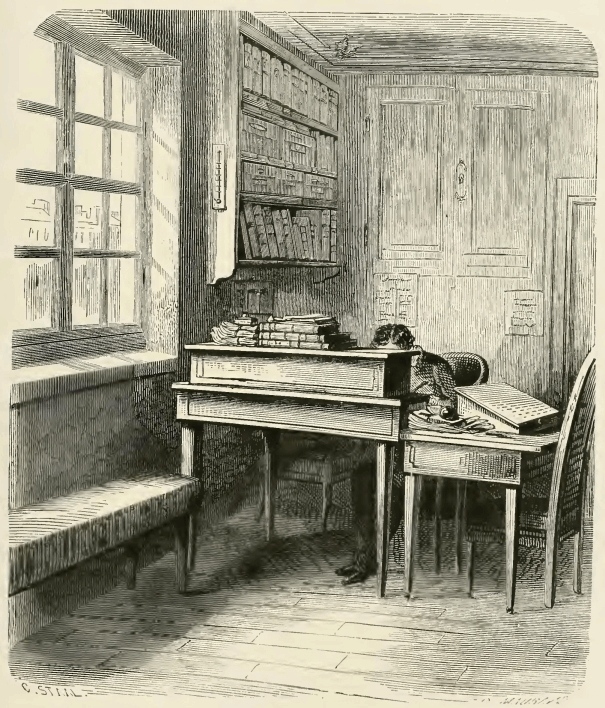
\includegraphics[width=\textwidth]{30261m.jpg}
\end{figure}

“It is a long time, madame,” said the procureur, describing a
half-circle with his chair, so as to place himself exactly opposite to
Madame Danglars,—“it is a long time since I had the pleasure of
speaking alone with you, and I regret that we have only now met to
enter upon a painful conversation.”

“Nevertheless, sir, you see I have answered your first appeal, although
certainly the conversation must be much more painful for me than for
you.” Villefort smiled bitterly.

“It is true, then,” he said, rather uttering his thoughts aloud than
addressing his companion,—“it is true, then, that all our actions leave
their traces—some sad, others bright—on our paths; it is true that
every step in our lives is like the course of an insect on the
sands;—it leaves its track! Alas, to many the path is traced by tears.”

“Sir,” said Madame Danglars, “you can feel for my emotion, can you not?
Spare me, then, I beseech you. When I look at this room,—whence so many
guilty creatures have departed, trembling and ashamed, when I look at
that chair before which I now sit trembling and ashamed,—oh, it
requires all my reason to convince me that I am not a very guilty woman
and you a menacing judge.”

Villefort dropped his head and sighed.

“And I,” he said, “I feel that my place is not in the judge’s seat, but
on the prisoner’s bench.”

\begin{figure}[ht]
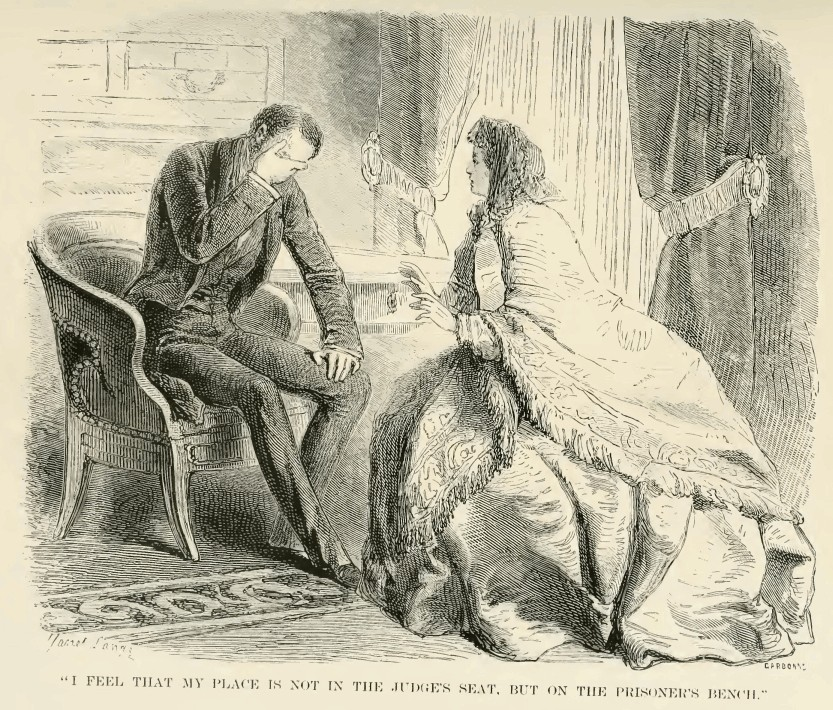
\includegraphics[width=\textwidth]{30263m.jpg}
\end{figure}

“You?” said Madame Danglars.

“Yes, I.”

“I think, sir, you exaggerate your situation,” said Madame Danglars,
whose beautiful eyes sparkled for a moment. “The paths of which you
were just speaking have been traced by all young men of ardent
imaginations. Besides the pleasure, there is always remorse from the
indulgence of our passions, and, after all, what have you men to fear
from all this? the world excuses, and notoriety ennobles you.”

“Madame,” replied Villefort, “you know that I am no hypocrite, or, at
least, that I never deceive without a reason. If my brow be severe, it
is because many misfortunes have clouded it; if my heart be petrified,
it is that it might sustain the blows it has received. I was not so in
my youth, I was not so on the night of the betrothal, when we were all
seated around a table in the Rue du Cours at Marseilles. But since then
everything has changed in and about me; I am accustomed to brave
difficulties, and, in the conflict to crush those who, by their own
free will, or by chance, voluntarily or involuntarily, interfere with
me in my career. It is generally the case that what we most ardently
desire is as ardently withheld from us by those who wish to obtain it,
or from whom we attempt to snatch it. Thus, the greater number of a
man’s errors come before him disguised under the specious form of
necessity; then, after error has been committed in a moment of
excitement, of delirium, or of fear, we see that we might have avoided
and escaped it. The means we might have used, which we in our blindness
could not see, then seem simple and easy, and we say, ‘Why did I not do
this, instead of that?’ Women, on the contrary, are rarely tormented
with remorse; for the decision does not come from you,—your misfortunes
are generally imposed upon you, and your faults the results of others’
crimes.”

“In any case, sir, you will allow,” replied Madame Danglars, “that,
even if the fault were alone mine, I last night received a severe
punishment for it.”

“Poor thing,” said Villefort, pressing her hand, “it was too severe for
your strength, for you were twice overwhelmed, and yet——”

“Well?”

“Well, I must tell you. Collect all your courage, for you have not yet
heard all.”

“Ah,” exclaimed Madame Danglars, alarmed, “what is there more to hear?”

“You only look back to the past, and it is, indeed, bad enough. Well,
picture to yourself a future more gloomy still—certainly frightful,
perhaps sanguinary!”

The baroness knew how calm Villefort naturally was, and his present
excitement frightened her so much that she opened her mouth to scream,
but the sound died in her throat.

“How has this terrible past been recalled?” cried Villefort; “how is it
that it has escaped from the depths of the tomb and the recesses of our
hearts, where it was buried, to visit us now, like a phantom, whitening
our cheeks and flushing our brows with shame?”

“Alas,” said Hermine, “doubtless it is chance.”

“Chance?” replied Villefort; “No, no, madame, there is no such thing as
chance.”

“Oh, yes; has not a fatal chance revealed all this? Was it not by
chance the Count of Monte Cristo bought that house? Was it not by
chance he caused the earth to be dug up? Is it not by chance that the
unfortunate child was disinterred under the trees?—that poor innocent
offspring of mine, which I never even kissed, but for whom I wept many,
many tears. Ah, my heart clung to the count when he mentioned the dear
spoil found beneath the flowers.”

“Well, no, madame,—this is the terrible news I have to tell you,” said
Villefort in a hollow voice—“no, nothing was found beneath the flowers;
there was no child disinterred—no. You must not weep, no, you must not
groan, you must tremble!”

“What can you mean?” asked Madame Danglars, shuddering.

“I mean that M. de Monte Cristo, digging underneath these trees, found
neither skeleton nor chest, because neither of them was there!”

“Neither of them there?” repeated Madame Danglars, her staring,
wide-open eyes expressing her alarm. “Neither of them there!” she again
said, as though striving to impress herself with the meaning of the
words which escaped her.

“No,” said Villefort, burying his face in his hands, “no, a hundred
times no!”

“Then you did not bury the poor child there, sir? Why did you deceive
me? Where did you place it? tell me—where?”

“There! But listen to me—listen—and you will pity me who has for twenty
years alone borne the heavy burden of grief I am about to reveal,
without casting the least portion upon you.”

“Oh, you frighten me! But speak; I will listen.”

“You recollect that sad night, when you were half-expiring on that bed
in the red damask room, while I, scarcely less agitated than you,
awaited your delivery. The child was born, was given to me—motionless,
breathless, voiceless; we thought it dead.”

Madame Danglars moved rapidly, as though she would spring from her
chair, but Villefort stopped, and clasped his hands as if to implore
her attention.

“We thought it dead,” he repeated; “I placed it in the chest, which was
to take the place of a coffin; I descended to the garden, I dug a hole,
and then flung it down in haste. Scarcely had I covered it with earth,
when the arm of the Corsican was stretched towards me; I saw a shadow
rise, and, at the same time, a flash of light. I felt pain; I wished to
cry out, but an icy shiver ran through my veins and stifled my voice; I
fell lifeless, and fancied myself killed. Never shall I forget your
sublime courage, when, having returned to consciousness, I dragged
myself to the foot of the stairs, and you, almost dying yourself, came
to meet me. We were obliged to keep silent upon the dreadful
catastrophe. You had the fortitude to regain the house, assisted by
your nurse. A duel was the pretext for my wound. Though we scarcely
expected it, our secret remained in our own keeping alone. I was taken
to Versailles; for three months I struggled with death; at last, as I
seemed to cling to life, I was ordered to the South. Four men carried
me from Paris to Châlons, walking six leagues a day; Madame de
Villefort followed the litter in her carriage. At Châlons I was put
upon the Saône, thence I passed on to the Rhône, whence I descended,
merely with the current, to Arles; at Arles I was again placed on my
litter, and continued my journey to Marseilles. My recovery lasted six
months. I never heard you mentioned, and I did not dare inquire for
you. When I returned to Paris, I learned that you, the widow of M. de
Nargonne, had married M. Danglars.

“What was the subject of my thoughts from the time consciousness
returned to me? Always the same—always the child’s corpse, coming every
night in my dreams, rising from the earth, and hovering over the grave
with menacing look and gesture. I inquired immediately on my return to
Paris; the house had not been inhabited since we left it, but it had
just been let for nine years. I found the tenant. I pretended that I
disliked the idea that a house belonging to my wife’s father and mother
should pass into the hands of strangers. I offered to pay them for
cancelling the lease; they demanded 6,000 francs. I would have given
10,000—I would have given 20,000. I had the money with me; I made the
tenant sign the deed of resilition, and when I had obtained what I so
much wanted, I galloped to Auteuil. No one had entered the house since
I had left it.

“It was five o’clock in the afternoon; I ascended into the red room,
and waited for night. There all the thoughts which had disturbed me
during my year of constant agony came back with double force. The
Corsican, who had declared the vendetta against me, who had followed me
from Nîmes to Paris, who had hid himself in the garden, who had struck
me, had seen me dig the grave, had seen me inter the child,—he might
become acquainted with your person,—nay, he might even then have known
it. Would he not one day make you pay for keeping this terrible secret?
Would it not be a sweet revenge for him when he found that I had not
died from the blow of his dagger? It was therefore necessary, before
everything else, and at all risks, that I should cause all traces of
the past to disappear—that I should destroy every material vestige; too
much reality would always remain in my recollection. It was for this I
had annulled the lease—it was for this I had come—it was for this I was
waiting.

“Night arrived; I allowed it to become quite dark. I was without a
light in that room; when the wind shook all the doors, behind which I
continually expected to see some spy concealed, I trembled. I seemed
everywhere to hear your moans behind me in the bed, and I dared not
turn around. My heart beat so violently that I feared my wound would
open. At length, one by one, all the noises in the neighborhood ceased.
I understood that I had nothing to fear, that I should neither be seen
nor heard, so I decided upon descending to the garden.

“Listen, Hermine; I consider myself as brave as most men, but when I
drew from my breast the little key of the staircase, which I had found
in my coat—that little key we both used to cherish so much, which you
wished to have fastened to a golden ring—when I opened the door, and
saw the pale moon shedding a long stream of white light on the spiral
staircase like a spectre, I leaned against the wall, and nearly
shrieked. I seemed to be going mad. At last I mastered my agitation. I
descended the staircase step by step; the only thing I could not
conquer was a strange trembling in my knees. I grasped the railings; if
I had relaxed my hold for a moment, I should have fallen. I reached the
lower door. Outside this door a spade was placed against the wall; I
took it, and advanced towards the thicket. I had provided myself with a
dark lantern. In the middle of the lawn I stopped to light it, then I
continued my path.

“It was the end of November, all the verdure of the garden had
disappeared, the trees were nothing more than skeletons with their long
bony arms, and the dead leaves sounded on the gravel under my feet. My
terror overcame me to such a degree as I approached the thicket, that I
took a pistol from my pocket and armed myself. I fancied continually
that I saw the figure of the Corsican between the branches. I examined
the thicket with my dark lantern; it was empty. I looked carefully
around; I was indeed alone,—no noise disturbed the silence but the owl,
whose piercing cry seemed to be calling up the phantoms of the night. I
tied my lantern to a forked branch I had noticed a year before at the
precise spot where I stopped to dig the hole.

“The grass had grown very thickly there during the summer, and when
autumn arrived no one had been there to mow it. Still one place where
the grass was thin attracted my attention; it evidently was there I had
turned up the ground. I went to work. The hour, then, for which I had
been waiting during the last year had at length arrived. How I worked,
how I hoped, how I struck every piece of turf, thinking to find some
resistance to my spade! But no, I found nothing, though I had made a
hole twice as large as the first. I thought I had been deceived—had
mistaken the spot. I turned around, I looked at the trees, I tried to
recall the details which had struck me at the time. A cold, sharp wind
whistled through the leafless branches, and yet the drops fell from my
forehead. I recollected that I was stabbed just as I was trampling the
ground to fill up the hole; while doing so I had leaned against a
laburnum; behind me was an artificial rockery, intended to serve as a
resting-place for persons walking in the garden; in falling, my hand,
relaxing its hold of the laburnum, felt the coldness of the stone. On
my right I saw the tree, behind me the rock. I stood in the same
attitude, and threw myself down. I rose, and again began digging and
enlarging the hole; still I found nothing, nothing—the chest was no
longer there!”

\begin{figure}[ht]
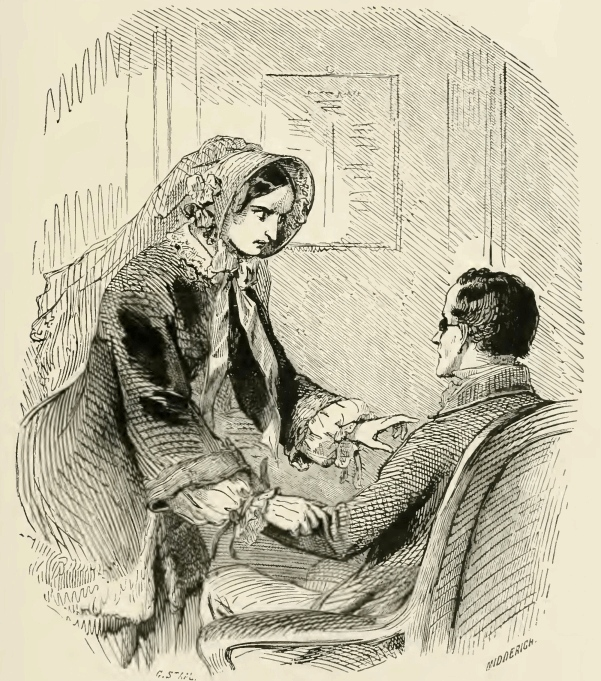
\includegraphics[width=\textwidth]{30269m.jpg}
\end{figure}

“The chest no longer there?” murmured Madame Danglars, choking with
fear.

“Think not I contented myself with this one effort,” continued
Villefort. “No; I searched the whole thicket. I thought the assassin,
having discovered the chest, and supposing it to be a treasure, had
intended carrying it off, but, perceiving his error, had dug another
hole, and deposited it there; but I could find nothing. Then the idea
struck me that he had not taken these precautions, and had simply
thrown it in a corner. In the last case I must wait for daylight to
renew my search. I remained in the room and waited.”

“Oh, Heaven!”

\begin{figure}[ht]
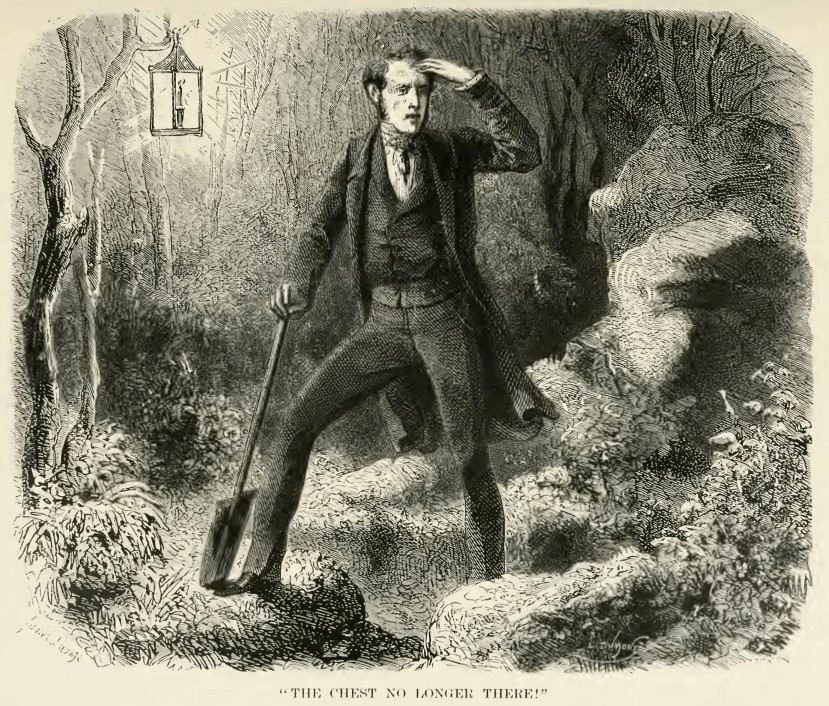
\includegraphics[width=\textwidth]{30271m.jpg}
\end{figure}

When daylight dawned I went down again. My first visit was to the
thicket. I hoped to find some traces which had escaped me in the
darkness. I had turned up the earth over a surface of more than twenty
feet square, and a depth of two feet. A laborer would not have done in
a day what occupied me an hour. But I could find nothing—absolutely
nothing. Then I renewed the search. Supposing it had been thrown aside,
it would probably be on the path which led to the little gate; but this
examination was as useless as the first, and with a bursting heart I
returned to the thicket, which now contained no hope for me.”

“Oh,” cried Madame Danglars, “it was enough to drive you mad!”

“I hoped for a moment that it might,” said Villefort; “but that
happiness was denied me. However, recovering my strength and my ideas,
‘Why,’ said I, ‘should that man have carried away the corpse?’”

“But you said,” replied Madame Danglars, “he would require it as a
proof.”

“Ah, no, madame, that could not be. Dead bodies are not kept a year;
they are shown to a magistrate, and the evidence is taken. Now, nothing
of the kind has happened.”

“What then?” asked Hermine, trembling violently.

“Something more terrible, more fatal, more alarming for us—the child
was, perhaps, alive, and the assassin may have saved it!”

Madame Danglars uttered a piercing cry, and, seizing Villefort’s hands,
exclaimed, “My child was alive?” said she; “you buried my child alive?
You were not certain my child was dead, and you buried it? Ah——”

Madame Danglars had risen, and stood before the procureur, whose hands
she wrung in her feeble grasp.

“I know not; I merely suppose so, as I might suppose anything else,”
replied Villefort with a look so fixed, it indicated that his powerful
mind was on the verge of despair and madness.

“Ah, my child, my poor child!” cried the baroness, falling on her
chair, and stifling her sobs in her handkerchief. Villefort, becoming
somewhat reassured, perceived that to avert the maternal storm
gathering over his head, he must inspire Madame Danglars with the
terror he felt.

“You understand, then, that if it were so,” said he, rising in his
turn, and approaching the baroness, to speak to her in a lower tone,
“we are lost. This child lives, and someone knows it lives—someone is
in possession of our secret; and since Monte Cristo speaks before us of
a child disinterred, when that child could not be found, it is he who
is in possession of our secret.”

“Just God, avenging God!” murmured Madame Danglars.

Villefort’s only answer was a stifled groan.

“But the child—the child, sir?” repeated the agitated mother.

“How I have searched for him,” replied Villefort, wringing his hands;
“how I have called him in my long sleepless nights; how I have longed
for royal wealth to purchase a million of secrets from a million of
men, and to find mine among them! At last, one day, when for the
hundredth time I took up my spade, I asked myself again and again what
the Corsican could have done with the child. A child encumbers a
fugitive; perhaps, on perceiving it was still alive, he had thrown it
into the river.”

“Impossible!” cried Madame Danglars: “a man may murder another out of
revenge, but he would not deliberately drown a child.”

“Perhaps,” continued Villefort, “he had put it in the foundling
hospital.”

“Oh, yes, yes,” cried the baroness; “my child is there!”

“I ran to the hospital, and learned that the same night—the night of
the 20th of September—a child had been brought there, wrapped in part
of a fine linen napkin, purposely torn in half. This portion of the
napkin was marked with half a baron’s crown, and the letter H.”

“Truly, truly,” said Madame Danglars, “all my linen is marked thus;
Monsieur de Nargonne was a baron, and my name is Hermine. Thank God, my
child was not then dead!”

“No, it was not dead.”

“And you can tell me so without fearing to make me die of joy? Where is
the child?”

Villefort shrugged his shoulders.

“Do I know?” said he; “and do you believe that if I knew I would relate
to you all its trials and all its adventures as would a dramatist or a
novel writer? Alas, no, I know not. A woman, about six months after,
came to claim it with the other half of the napkin. This woman gave all
the requisite particulars, and it was intrusted to her.”

“But you should have inquired for the woman; you should have traced
her.”

“And what do you think I did? I feigned a criminal process, and
employed all the most acute bloodhounds and skilful agents in search of
her. They traced her to Châlons, and there they lost her.”

“They lost her?”

“Yes, forever.”

Madame Danglars had listened to this recital with a sigh, a tear, or a
shriek for every detail. “And this is all?” said she; “and you stopped
there?”

“Oh, no,” said Villefort; “I never ceased to search and to inquire.
However, the last two or three years I had allowed myself some respite.
But now I will begin with more perseverance and fury than ever, since
fear urges me, not my conscience.”

“But,” replied Madame Danglars, “the Count of Monte Cristo can know
nothing, or he would not seek our society as he does.”

“Oh, the wickedness of man is very great,” said Villefort, “since it
surpasses the goodness of God. Did you observe that man’s eyes while he
was speaking to us?”

“No.”

“But have you ever watched him carefully?”

“Doubtless he is capricious, but that is all; one thing alone struck
me,—of all the exquisite things he placed before us, he touched
nothing. I might have suspected he was poisoning us.”

“And you see you would have been deceived.”

“Yes, doubtless.”

“But believe me, that man has other projects. For that reason I wished
to see you, to speak to you, to warn you against everyone, but
especially against him. Tell me,” cried Villefort, fixing his eyes more
steadfastly on her than he had ever done before, “did you ever reveal
to anyone our connection?”

“Never, to anyone.”

“You understand me,” replied Villefort, affectionately; “when I say
anyone,—pardon my urgency,—to anyone living I mean?”

“Yes, yes, I understand very well,” ejaculated the baroness; “never, I
swear to you.”

“Were you ever in the habit of writing in the evening what had
transpired in the morning? Do you keep a journal?”

“No, my life has been passed in frivolity; I wish to forget it myself.”

“Do you talk in your sleep?”

\begin{figure}[ht]
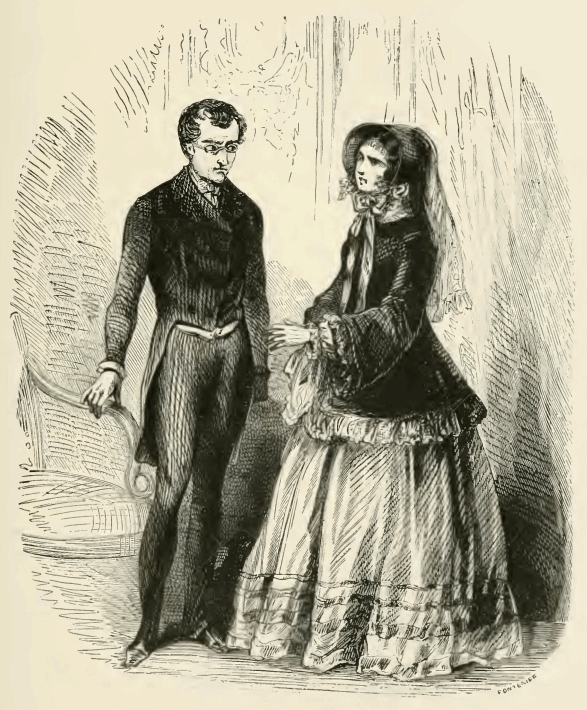
\includegraphics[width=\textwidth]{30275m.jpg}
\end{figure}

“I sleep soundly, like a child; do you not remember?”

The color mounted to the baroness’s face, and Villefort turned awfully
pale.

“It is true,” said he, in so low a tone that he could hardly be heard.

“Well?” said the baroness.

“Well, I understand what I now have to do,” replied Villefort. “In less
than one week from this time I will ascertain who this M. de Monte
Cristo is, whence he comes, where he goes, and why he speaks in our
presence of children that have been disinterred in a garden.”

Villefort pronounced these words with an accent which would have made
the count shudder had he heard him. Then he pressed the hand the
baroness reluctantly gave him, and led her respectfully back to the
door. Madame Danglars returned in another cab to the passage, on the
other side of which she found her carriage, and her coachman sleeping
peacefully on his box while waiting for her.
